\begin{fullwidth}
    \section{Trading Rewards} \label{sec:incentives}

    \begin{adjustwidth}{2cm}{2cm}
        \justify
        Two key incentives programs for dYdX v3 were Trading Rewards and Liquidity Provider (LP) Rewards. Recent changes have led to a transition away from LP Rewards and towards Market Maker rebates, which we touched on briefly in Section \ref{sec:validators}. Conversely, trading rewards will remain a cornerstone of dYdX's ecosystem incentives with dYdX v4. The new module boasts two key parameters that the community must manage effectively to promote growth in the ecosystem, while avoiding excessive spending. In this section we discuss the new trading rewards mechanics and provide a tentative framework for managing them moving forward.
    \end{adjustwidth}
    
    \textcolor{gray}{\rule{\linewidth}{0.1mm}}
\end{fullwidth}

    The trading rewards module has undergone several changes since its inception in 2021. In the following subsections, we will provide a brief history of trading rewards on dYdX v3, an overview of the new trading rewards mechanism on dYdX v4, and finally an experimental design framework for managing v4 Trading Rewards parameters. Part of our framework hinges on preventing wash traders from profitably farming the trading rewards module. Our wash trading analysis can be found in Appendix \ref{app:wash}.

    \subsection{A Brief History of v3 Trading Rewards}

        At its inception in August of 2021, dYdX's Trading Rewards program would disburse ethDYDX according to the following formula:

        \begin{equation}
            r_i = R \cdot \frac{w_i}{\sum_n{w_n}},
        \end{equation}

        where $r_i$ is the rewards disbursed to the $i^{\text{th}}$ trader, $w_i$ is that trader's ``weight'' compared to other traders, and $R$ is the total rewards being distributed over the 28-day measurement period, called an epoch. A trader's weight was calculated as:

        \begin{equation}
            w_i = f^{0.7} \cdot d^{0.3},
        \end{equation}

        where $f$ is the fees paid by trader $i$ over the epoch, and $d$ was the average open interest they held. This weight function, commonly known as a Cobb-Douglas utility function, aimed to increase the number of outstanding derivatives contracts held on dYdX v3. \sidenotequote{After the launch of the token, dYdX trading volumes skyrocketed to over \$2B / day.}{\bhref{https://antonio-dydx.medium.com/the-history-of-dydx-so-far-68bf46789f86}{The History of dYdX (so far) - Antonio Juliano, CEO dYdX}}

        This early iteration of the Trading Rewards liquidity mining program was successful in driving exchange volume and open interest and garnered attention from institutional and retail traders alike. However, it had one undesirable side-effect: it was susceptible to ``farming''. 
        
        Sophisticated agents quickly identified ways to extract more value from the trading rewards program than they spent in fees in a given epoch. An extreme example of this is wash trading: throughout the earlier epochs of the Trading Rewards program, many addresses were caught trading between two accounts held by the same entity in order to avoid paying the bid-ask spread. The dYdX Foundation, the progenitors of the ethDYDX token and the Trading Rewards program, quickly identified this problem and blacklisted addresses caught wash trading.

        However, wash trading was not the only strategy traders used to farm dYdX's rewards program. In a \bhref{https://xenophonlabs.com/papers/dydx_trade_rewards.pdf}{research paper} published in early 2022, Xenophon Labs identified strategies for how traders might profit from the rewards program by optimizing market-neutral positions. 
        
        Our analysis pointed to a few undesirable properties of the Trading Rewards program:

        \begin{itemize}
            \item The complexity of the Cobb-Douglas function benefited skilled traders that (a) had the resources to maintain high open interest throughout an epoch and (b) had the technical sophistication to avoid liquidations and optimize their fees paid to maximize profits. This further incentivized the creation of leveraged, hedged positions that maximized open interest without accepting any market risk. The profits of these sophisticated traders came at the expense of retail traders who ended up receiving less rewards.
            \item The program seemed to be attracting ``mercenary'' traders, instead of ``sticky'' or loyal users; as the price of ethDYDX plummeted throughout late 2021 and early 2022, the fees paid on dYdX v3 plummeted accordingly. See Fig. \ref{fig:fee_correlation}. Given that the ethDYDX supply is limited, users acquired through the Trading Rewards program should ideally remain on the platform even as incentives declined. 
        \end{itemize}

        \begin{figure}[htp]
            \centering
            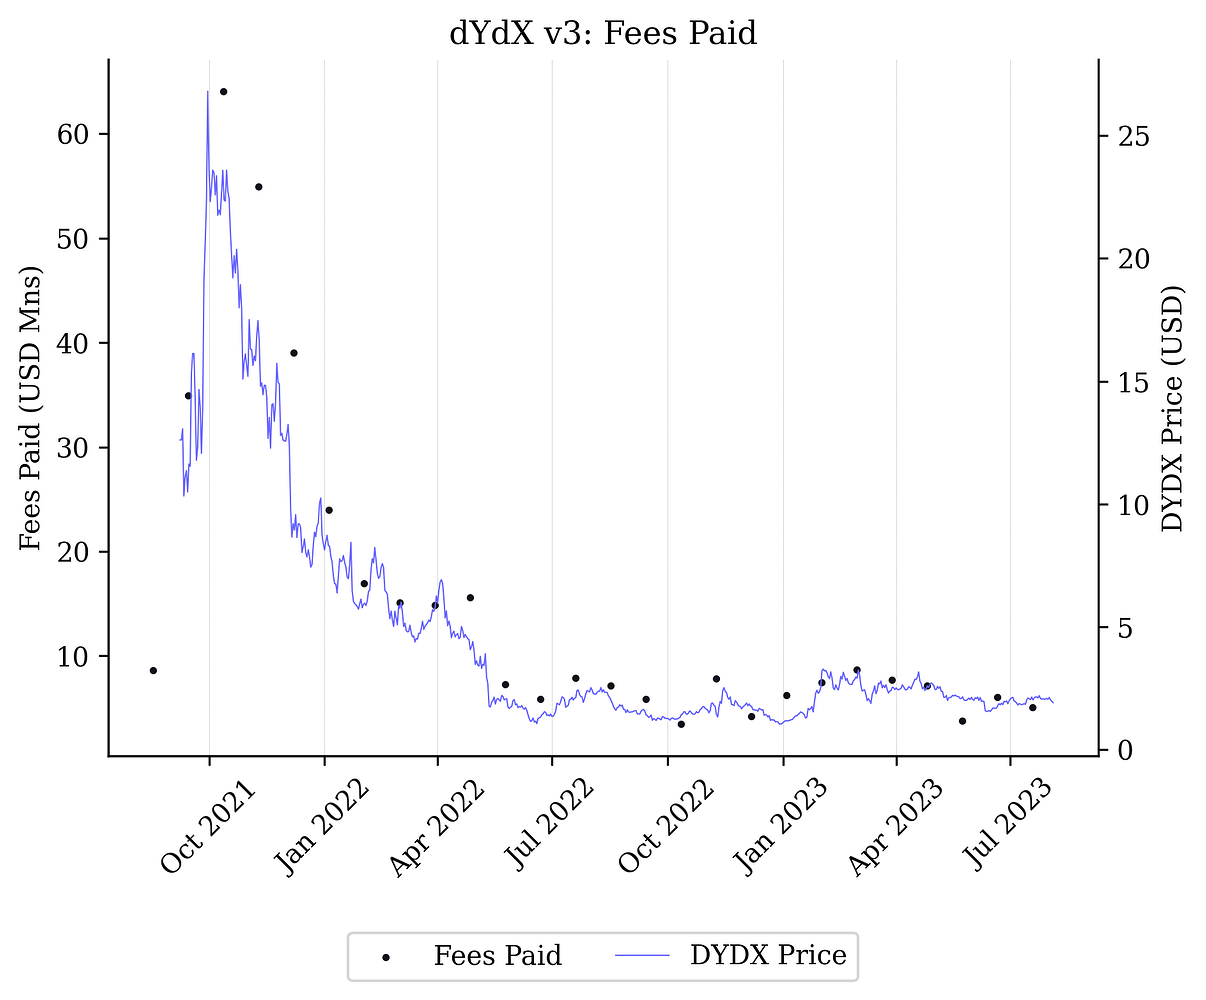
\includegraphics[width=0.7\linewidth]{figs/fee_correlation.png}
            \caption{This plot compares the fees paid on the dYdX v3 platform to the price of ethDYDX token. Notice that fees paid are highly correlated with ethDYDX token price, indicating that a large cohort of traders are sensitive to the Trading and LP rewards programs.}
            \label{fig:fee_correlation}
        \end{figure}

        In the months that followed, several governance proposals were submitted to address both concerns. See their chronology below:

        \begin{itemize}
            \item April 2022: Increase the weight of fees, decrease the weight of open interest in the Trading Rewards formula. Proposed by Xenophon Labs. See the discussion \bhref{https://forums.dydx.community/discussion/4190-discussion-dydx-trader-rewards-mechanism-review}{here}.
            \item August 2022: Simplify the rewards formula to only account for fees paid. Proposed by SLN Capital. See the discussion \bhref{https://forums.dydx.community/discussion/6324-discussion-revisionssimplification-of-trading-rewards}{here}.
            \item September 2022: Reduce trading rewards by 25\%. Proposed by Wintermute governance. See the discussion \bhref{https://forums.dydx.community/discussion/6324-discussion-revisionssimplification-of-trading-rewards}{here}.
            \item February 2023: Further reduce trading rewards by 45\%. Proposed by Wintermute governance. See the discussion \bhref{https://forums.dydx.community/discussion/9949-drc-reduce-trading-rewards-by-45}{here}.
        \end{itemize}

        The simplification of the rewards formula, first by reducing the weight of open interest, then by eliminating open interest entirely, served to make the program more equitable for retail traders, and reduce the marginal advantage (or edge) available to sophisticated traders in maximizing their profits from rewards. The reduction in trading rewards expenditure served to make the program more sustainable as the protocol matured and more evidence was gathered that the program was largely attracting mercenary volume. 

        \begin{figure}[htp]
            \centering
            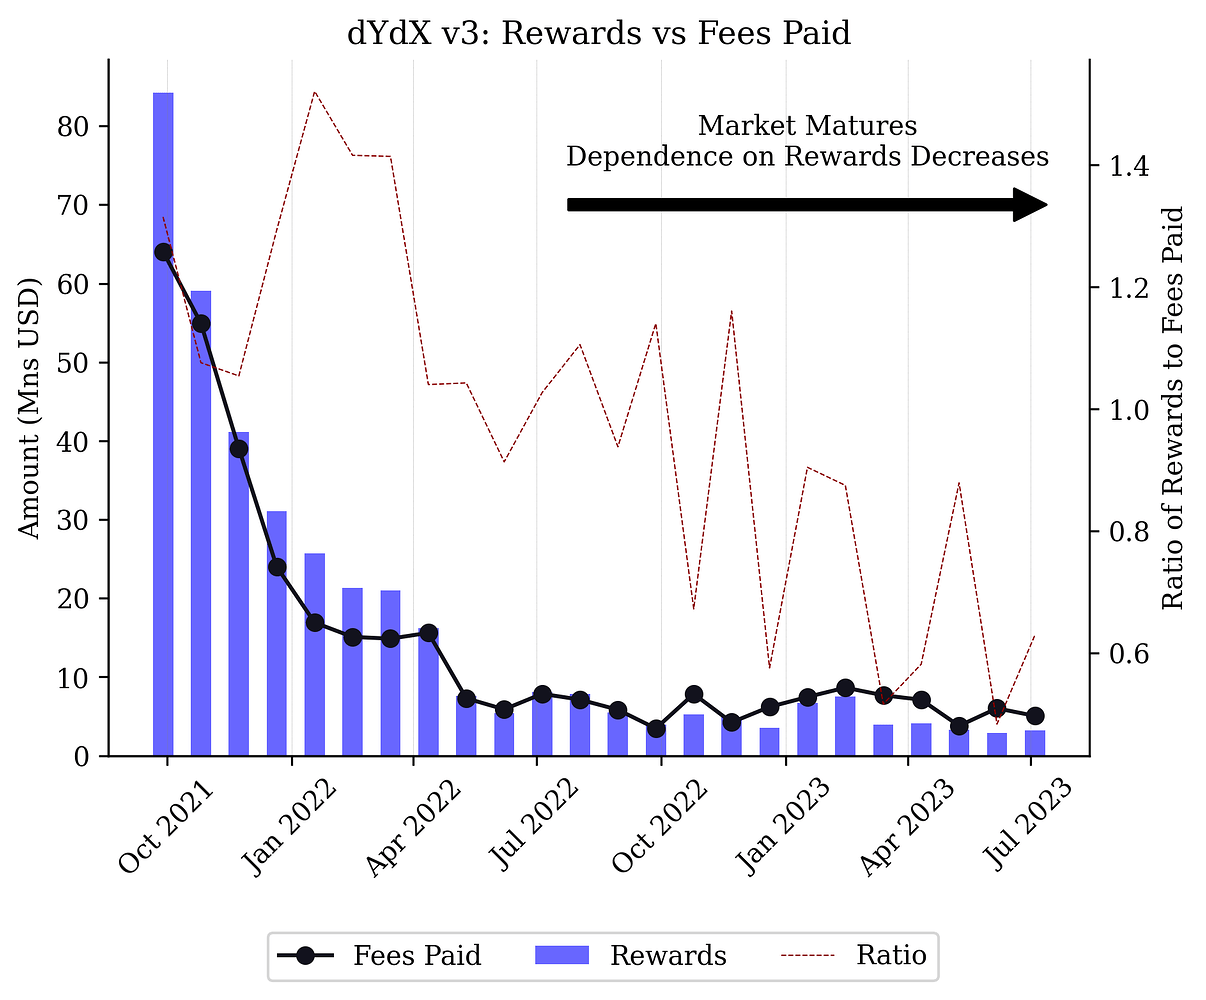
\includegraphics[width=0.7\linewidth]{figs/v3_rewards_analysis.png}
            \caption{This plot compares the fees paid on dYdX v3 to the amount spent in rewards. Notice that dYdX was paying more in rewards than it was earning in fees throughout earlier epochs. As the market matured and several governance proposals amended the rewards program, trading activity became less sensitive to the value of rewards being disbursed.}
            \label{fig:v3_rewards_analysis}
        \end{figure}

    \subsection{Overview of v4 Trading Rewards}
    
        An opportunity arose to improve upon the v3 Trading Rewards program with the launch of dYdX v4\sidenote{See this \bhref{https://dydx.exchange/blog/v4-rewards-and-parameters}{announcement} by dYdX Trading on the new rewards formula, or this \bhref{https://dydx.forum/t/dydx-v3-vs-v4-new-trader-rewards-overview/881}{brief overview} by Xenophon Labs.}. First and foremost, while trading rewards on dYdX v3 were paid in 28-day cycles (epochs), v4 trading rewards will be paid at the end of every block, or roughly every two seconds. That is, each user is now immediately rewarded for paying fees to the protocol.

        Each block, a predetermined amount of DYDX is emitted to the rewards module to be distributed as rewards. Let's denote this amount as $E$, for emissions. At the end of the block, the following amount of DYDX is disbursed to traders by the trading rewards module:

        \begin{equation}
            A = \min{\left(C \cdot \frac{S}{p}, T\right)},
        \end{equation}

        where $A$ is the total amount of DYDX disbursed, $C \in [0, 1]$ is a community-owned parameter (originally set to $0$), $S$ is the total amount of fees paid to the protocol (adjusted by maker rebates), $p$ is the oracle price of DYDX token, and $T$ is the total amount of DYDX sitting in the rewards module. Notice that $T$ is the sum of the per-block emissions $E$ and the leftover DYDX that was not disbursed in the previous block.

        Herein lies a key difference between v3 rewards and v4 rewards. On dYdX v3, all emissions to the Trading Rewards module would be distributed to traders regardless of how much was paid in fees. As we saw on Fig. \ref{fig:v3_rewards_analysis}, this led to the protocol often disbursing more in rewards than it received in fees, particularly throughout earlier epochs when sophisticated traders could optimize their open interest to profit off the rewards program. 

        On dYdX v4, the rewards distributed at each block are limited not only by the amount of DYDX available in the rewards module, $T$, but also by the total amount of fees paid during that block, $S$. By managing the $C$ parameter, the community controls the maximum proportion of fees that may be rebated back to traders as DYDX rewards, and by ensuring that $C < 1$, the protocol never pays more in rewards than it earns in fees. \sidenotequote{Trading rewards should limit the protocol overspending on trading activity}{\bhref{https://dydx.exchange/blog/v4-rewards-and-parameters}{v4 Deep Dive: Rewards and Parameters}}

        At a high level, the $C$ parameter acts as a simple pricing lever for the community to make trading cheaper on dYdX v4 without damaging validator incentives. Instead of lowering fees, which would come at the expense of the chain's stakers and validators, the community may choose to enforce a high $C$ parameter. 

        At Genesis, the $C$ parameter will be set to $0\%$. The community may then choose to increase the $C$ parameter to enable trading rewards. The emissions to the trading rewards module have not yet been determined, and will depend on the amount of DYDX credited to the rewards vester account on dYdX Chain, which we discussed in Section \ref{subsubsec:upgrade}.

        Given that trading rewards consume a major portion of DYDX expenses (i.e., inflation) a crucial responsibility for the community is to adequately manage both the emissions to the module, and the maximum trading fee ``discount'' provided by the module, parameterized by $C$. In what follows, we provide a tentative framework for managing trading rewards parameters based on the principles of experimental design.
        
    \subsection{Managing Trading Rewards Parameters}
    
        The thesis for our parameter-setting framework is simple: \textit{it is exceptionally hard to optimize a protocol’s parameters without rich empirical data}. We believe the key to effectively managing dYdX Chain parameters, particularly trading rewards parameters, will be to construct these rich, empirical datasets through robust hypothesis testing. That is, we must make changes to trading rewards parameters and observe their effects on some key protocol metrics. Specifically, our framework aims to optimize Trading Rewards parameters against the program’s Gross Profits and/or Return On Investment (ROI).
        
        By iteratively modifying Trading Rewards parameters and observing how users react, we may build empirical user behavior models that we then leverage for future parameter adjustments. Ultimately, this experimental design framework will allow us to tend towards a locally optimal configuration of Trading Rewards with respect to our key metrics.\sidenote{In dYdX v3 the Trading Rewards parameters were changed only a handful of times, with little statistical analysis being published on the effects of these changes on trading volume. We are proposing this framework to avoid this pitfall with dYdX v4, and encourage the community to actively manage trading rewards parameters to nurture the ecosystem's growth and avoid over or under spending on the program.}

        The primary goal of this framework is to enforce statistical rigor when making and assessing changes to rewards programs. Previous proposals by Xenophon Labs and other dYdX contributors may have been directionally correct, but have not placed enough emphasis on a robust testing framework to (a) motivate the proposal, and (b) assess whether the proposal successfully improved a particular metric.

        \subsubsection{Metrics}

            We consider two key metrics that we believe lie at the core of the trading rewards program: gross profits and ROI. Gross profits are merely the protocol's revenue (or fees paid) minus the protocol's costs (or rewards). We formalize gross profits as:

            \begin{equation}
                \text{Gross Profits} := \text{Fees Paid} - \text{Rewards Emitted}.
            \end{equation}

            Denote $E = \text{Rewards Emitted}$ and $f(E, C) = \text{Fees Paid}$. Notice that fees paid is a function of both trading rewards parameters. We can rewrite gross profits as:

            \begin{equation}
                \text{Gross Profits} := f(C, E) - E.
            \end{equation}
            
            Similarly, ROI can be expressed as:

            \begin{equation}
                \text{ROI} := \frac{f(C, E) - E}{E}.
            \end{equation}

            The effective management of rewards parameters aims to maximize one of these metrics by gathering data on the curve $f(C, E)$. We can formalize this problem as: 

            \begin{align*}
                \text{maximize} &: \text{metric} \\ 
                \text{subject to} &: 0 < E < \text{Budget} 
            \end{align*}

            Whether to maximize profits or returns from the trading rewards program is a complex decision. Assuming that there is a positive relationship between the amount of DYDX emitted to the trading rewards program and the amount of fees being paid, a profit-maximization scheme would likely demand a greater investment into the trading rewards program. During the first several months of dYdX v4, the community might reasonably choose to spend more DYDX on an aggressive trading rewards program to accelerate growth and dominate the perpetuals market. However, as the protocol matures and the limit on DYDX inflation looms, the community might choose to pivot into an ROI-maximization scheme, which would likely demand a reduced expense on the Trading Rewards program to avoid spending DYDX past the point of diminishing returns.

            \begin{figure}[htp]
                \centering
                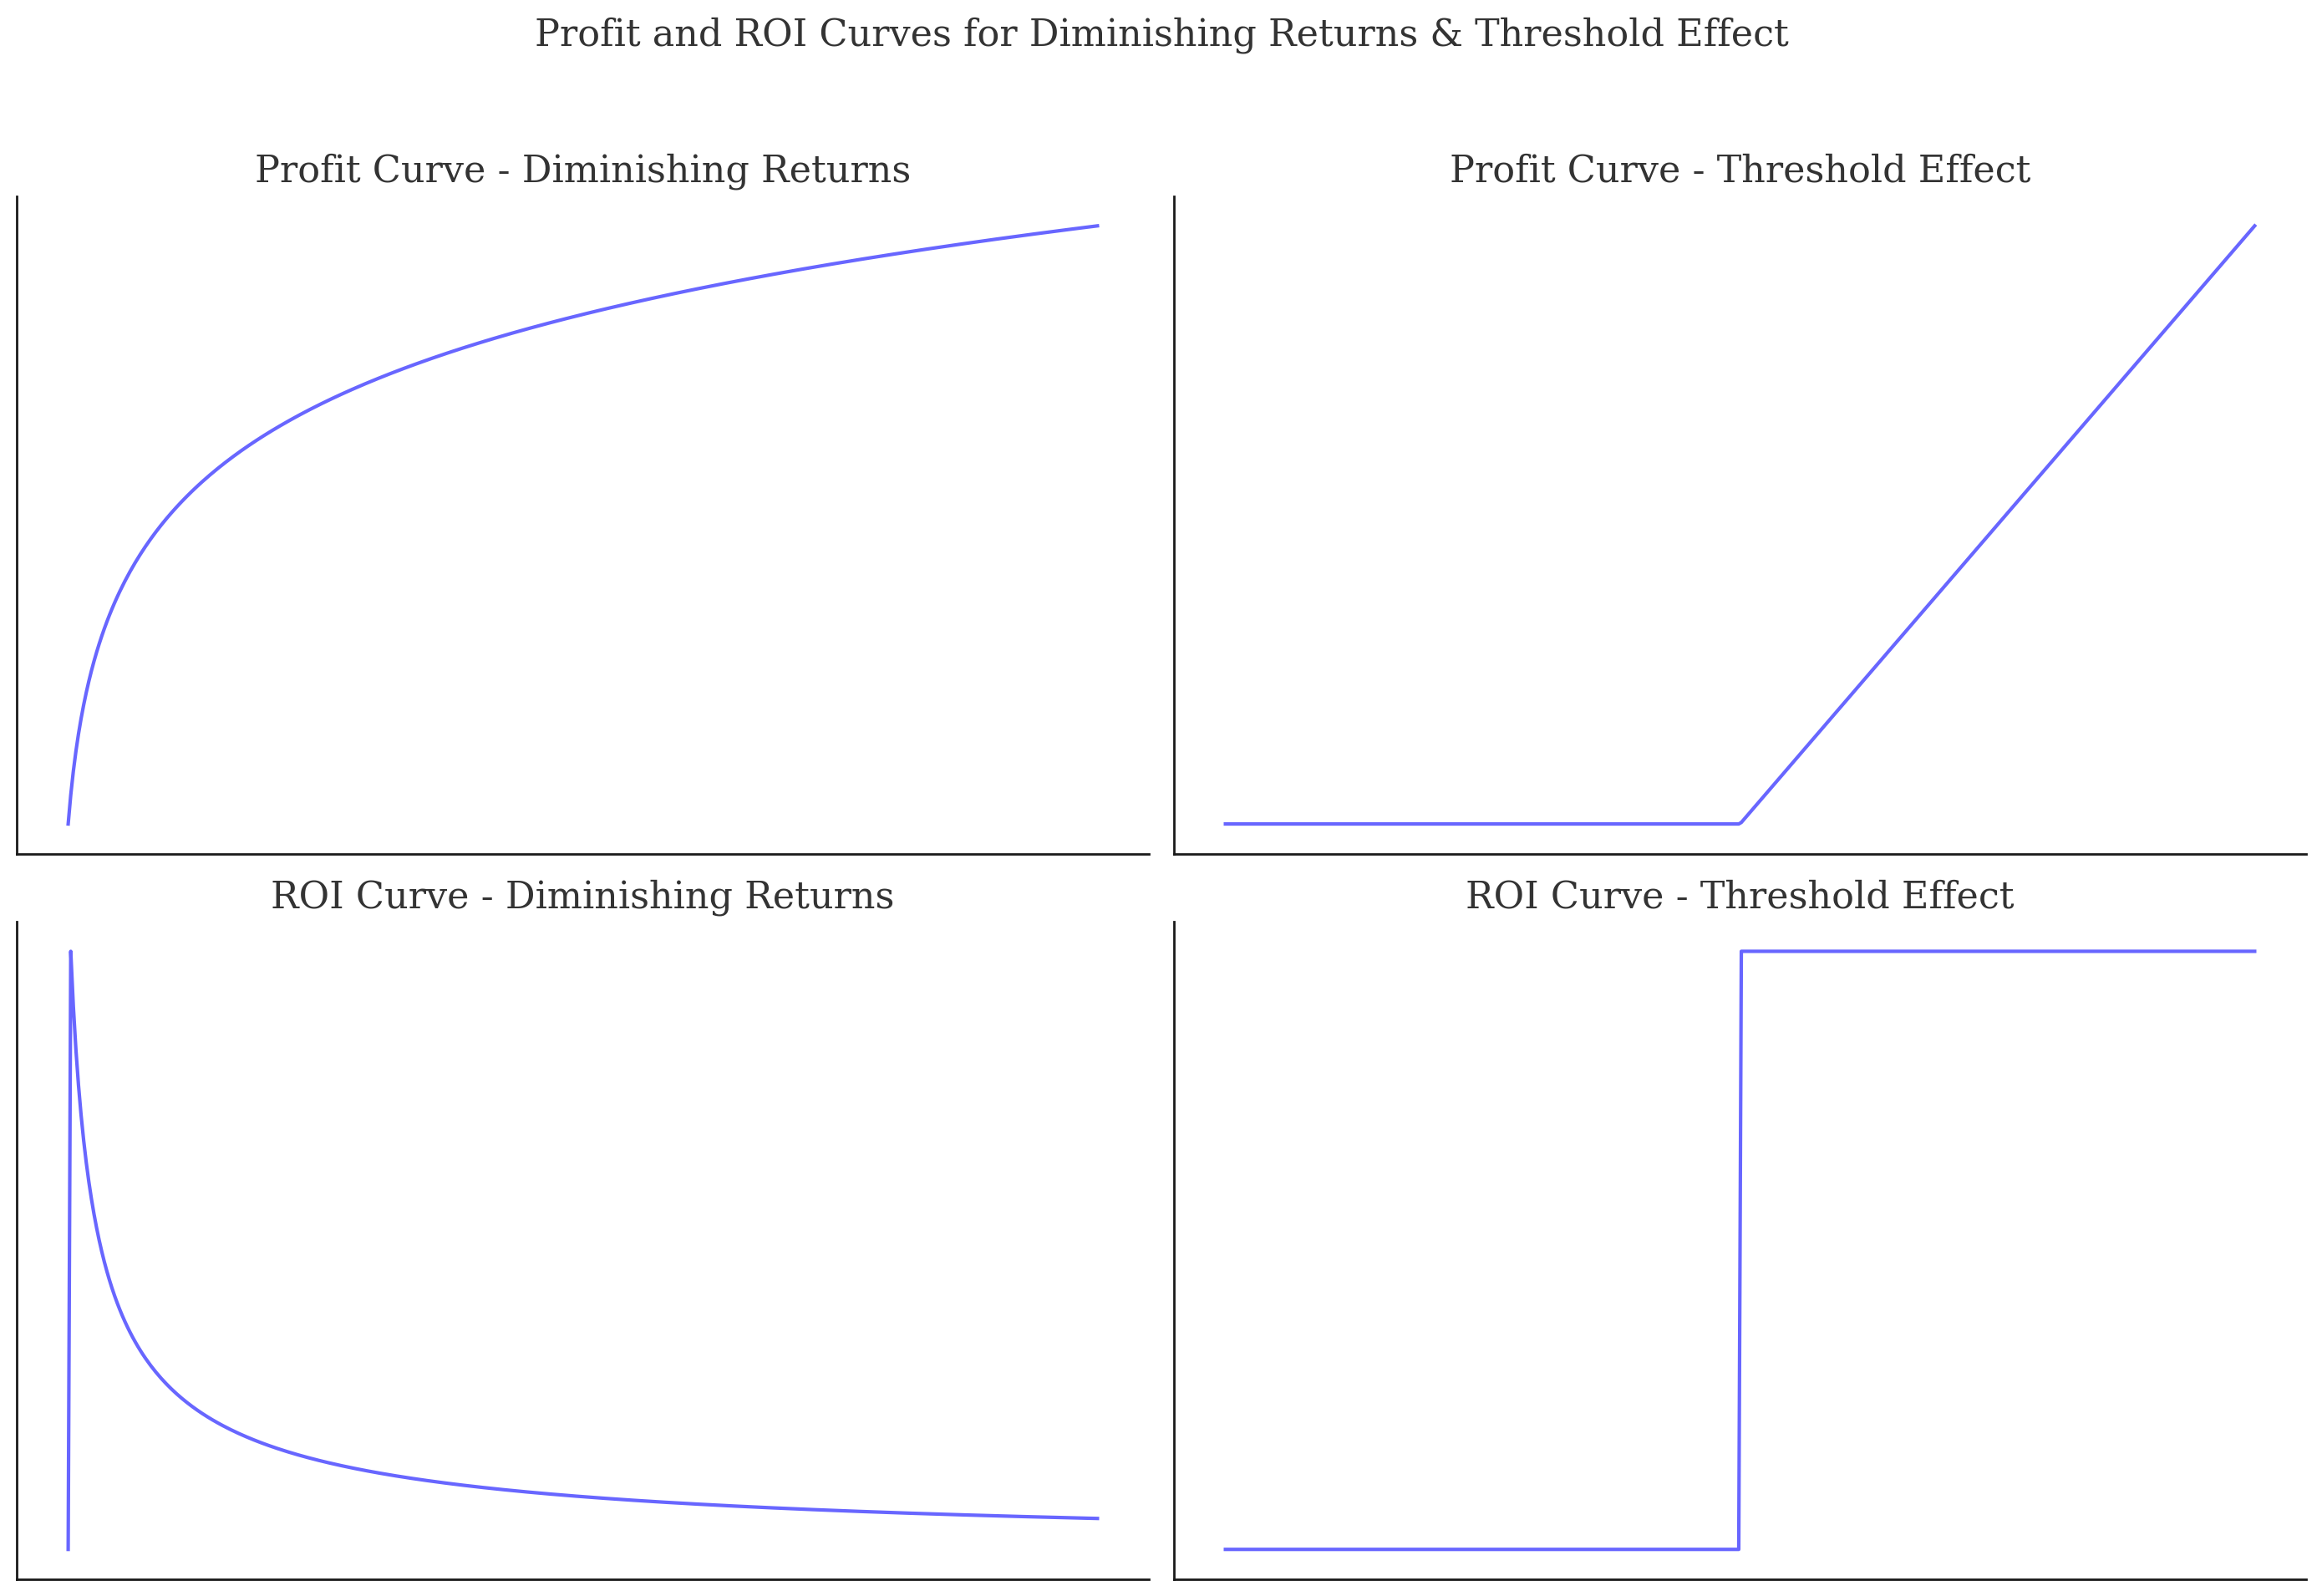
\includegraphics[width=\linewidth]{figs/roi_profit_curves.png}
                \caption{Simple examples for what the profit and ROI curves on the trading rewards program might look like.}
                \label{fig:roi_profit_curves}
            \end{figure}

        \subsubsection{Hypothesis Testing}

            Lets begin with a motivating example for how hypothesis testing may lead to significant efficiency improvements in the trading rewards program. Suppose the current trading rewards parameters are $\{C_0, E_0\}$, and we are considering lowering $C$ from $C_0$ to $C'$.

            \begin{align*}
                H_0 = \text{Lowering $C$ from $C_0$ to $C'$ has no statistically significant impact on the program's ROI.} \\
                H_a = \text{Lowering $C$ from $C_0$ to $C'$ has a statistically significant impact on the program's ROI.}
            \end{align*}

            More formally, we will be measuring the observed ROI during some sampling period before and after our change. For example, we may measure the ROI of the program at every block before we lower $C$ for $N$ blocks, comprising a period of approximately 2 weeks. We will repeat these measurements for $N$ blocks following the change to the $C$ parameter. Then, we may conduct a statistical test such as a paired t-test to determine whether the change to the program's ROI was statistically significant, accounting for the mean difference in ROI before and after the change, as well as the variance in measurements. If the results of our paired t-test fall within our confidence interval, which we may set to $95\%$, then we may determine that lowering $C$ does, indeed, lead to a meaningful change in the ROI of the trading rewards program. 

            Based on these results, we may proceed with some predetermined \textit{action}.

            \begin{itemize}
                \item \textbf{Success:} If lowering $C$ led to an improvement in the trading rewards program, we may choose to persist the change, and potentially continue to lower $C$ in the future.
                \item \textbf{Failure:} If lowering $C$ leads to a decrease in the program's ROI, we may choose to revert our change.
                \item \textbf{Inconclusive:} If lowering $C$ led to inconclusive results (i.e., we fail to reject the two-sided null hypothesis), then we may choose to wait and gather more data.
            \end{itemize}

            Although this is a simple example, it captures the essence of our experimental design framework:

            \begin{enumerate}
                \item \textbf{Parameter.} Choose a single variable to modify. Modifying multiple variables could lead to ambiguous conclusions.
                \item \textbf{Metric.} Choose an appropriate metric to test, such as return on investment.
                \item \textbf{Test.} Determine the statistical test to be used, such as a paired t-test to compare measurements across before-and-after samples.
                \item \textbf{Action.} Determine what to do if
                \begin{enumerate}
                    \item the parameter change led to an improvement in the metric: persist the change.
                    \item the parameter change led to a deterioration in the metric: revert the change. Requires an additional governance proposal. 
                    \item the null hypothesis was not rejected: extend the measurement period, or revert the change. 
                \end{enumerate}
            \end{enumerate}

            Intuitively, this hypothesis testing framework acts as a gradient-descent approach to optimizing the trading rewards module: we apply small changes to each individual parameter, if we observe that the change improves the appropriate metrics, we persist the change and, in the future, further change the parameter in the same direction. This way, we can gradually ``walk'' towards an optimal parameter configuration. 

            We consider the following constraints to our hypothesis testing framework:

            \begin{itemize}
                \item \textbf{Budget}. The community may choose to enforce a maximum budget on the emissions to the trading rewards module.
                \item \textbf{Maximum Changes}. The community may choose to enforce a maximum change to each parameter. For example, the $C$ parameter may not be changed by more than $5\%$ at a time.
                \item \textbf{Frequency}. The community may choose to enforce a maximum frequency for running these hypothesis tests. For example, these tests may not be run more frequently than once a month.
            \end{itemize}

        \subsubsection{Limitations}

            There is one obvious limitation to this approach: fees paid to the protocol are not exclusively functions of trading rewards parameters. This has two corollaries:

            \begin{itemize}
                \item \textbf{Spurious correlations:} hypothesis tests might indicate that a particular change was successful when the true reason a metric improved is due to a change in an external variable. The opposite might also be true, where a change to a parameter would have otherwise led to an improvement in a metric, but this was superceded by the effects of changes to an external variable. The proposer of a particular test must be transparent about confounding variables and how they may have affected the results of the test.
                \item \textbf{Non-Stationary Optimization:} the optimal configuration of trading rewards parameters may change over time due to external market conditions or user preferences. For example, it might be optimal for the community to support higher emissions on trading rewards throughout the early months of the exchange, and over time reduce these emissions as the product matures. The community should regularly review the program's metrics and, based on shifting market conditions, suggest adjustments to the parameters as needed.
            \end{itemize}

        \subsubsection{DYDX Price and Elasticity}

            One question the reader might have is how one would decide to experiment with higher or lower parameters. One way a community member might make this decision is by using a simpler measurement on the elasticity of traders to the trading rewards program.

            The community might be able to naturally observe whether traders on dYdX v4 are elastic or inelastic by comparing fees paid to the protocol with DYDX price. As DYDX price fluctuates, the dollar value of per-block rewards also fluctuates. If, over a meaningful period of time, a reduction to DYDX price does not lead to a reduction to fees being paid, the community may be fairly confident that demand on dYdX Chain is inelastic.

            Over time, data comparing fees paid to the protocol with the price of DYDX might be used to construct a curve $f(E, C, p)$, where $p$ is the price of DYDX. Assuming no changes to $E, C$, the curve $f(p)$ could offer insights on the elasticity of demand at different DYDX prices. 

            In the extremes, we might observe that traders are completely inelastic to the trading rewards program, in which case we might gradually reduce the program's emissions, test whether this hypothesis is true, and eventually wind down the program entirely.

            Of course, we find this would be a very unlikely outcome! In all likelihood, traders will be sensitive to both trading rewards parameters and to the price of DYDX. A more nuanced possibility is that, if DYDX price rises sharply, there is a point of diminishing returns where, despite increases in DYDX price (and therefore an increase in the dollar value of rewards distributed) fees don't continue increasing at the same rate. In this case, the community might choose to reduce emissions to avoid crossing the point of diminishing returns. 

    \subsection{On Wash Trading}

        One additional consideration for managing the trading rewards program is preventing wash trading from being profitable. At its surface, trading rewards is not a profitable wash trading opportunity since traders can never receive more in rewards than they pay in fees. However, traders on dYdX Chain might also be stakers. As stakers, they receive part of the fees paid to the protocol as staking rewards. A staker that commands a sufficient proportion of the chain's stake might be able to profitably wash trade on dYdX Chain, receiving more in trading plus staking incentives than they pay in fees.

        Additionally, these large stakers don't necessarily need to engage in wash trading to benefit from this dynamic. These stakers might simply be large traders on the chain, pushing significant volume from profitable trading strategies, or they might be sophisticated market makers with a large DYDX allocation. 

        In Appendix \ref{app:wash}, we discuss the profitability of self-trading with respect to trading and staking rewards, and the implications for setting trading rewards parameters.

    \subsection{Potential Improvement: Market Discrimination}

        Effective incentives programs often aim to identify which users are most price-sensitive and treat them accordingly. For example, ride-sharing apps might identify which users are most elastic to surge pricing and offer them additional discounts to keep them on their platform. 

        Although cryptocurrency protocols are often unable to discriminate between users, a problem referred to as ``Sybil resistance'', they may discriminate between the activities each user chooses to participate in.

        On dYdX Chain, a key differentiating factor between users is the market they choose to trade in. In a \bhref{https://drive.google.com/file/d/1g5te0E0jo76UvJw_lbmw5pvqSDJ6HtQd/view}{study} conducted by dYdX community members 0xCLR and 0xCChan, volume flowing through the BTC and ETH markets was found to be less elastic to trading fees than alternative, smaller markets like XRP or SOL. This creates an opportunity to price-discriminate between traders (or, more accurately, trades) flowing through these different markets, charging them according to their observed elasticity.

        Similarly, it might be prudent to increase or decrease the Trading Rewards allocated to different markets on dYdX Chain. For example, allocating a smaller share of rewards to the protocol's largest, most established markets might lead to negligible impact on the fees being paid to the protocol, since traders in these markets are not as sensitive to trading rewards. In turn, this would lead to an improved ROI for the program.

        At launch, the Trading Rewards program does not discriminate between markets. However, as dYdX Chain matures and engineering resources are freed up to conduct potential optimizations on incentives programs such as trading rewards, we might find it profitable to modify the trading rewards mechanism to incorporate discriminating factors such as markets.